\documentclass[tikz, border=7pt]{standalone}

\usepackage[T1]{fontenc}
\usepackage[english]{babel}


\usepackage{tikz,pgfplots}

%\usetikzlibrary{shapes, arrows, shadows, calc, decorations}

\usepackage{amsmath}

\begin{document}
    \pgfplotsset{every axis/.append style={
        font=\footnotesize,
        line width=1pt,
        tick style={ultra thin}}
    }
    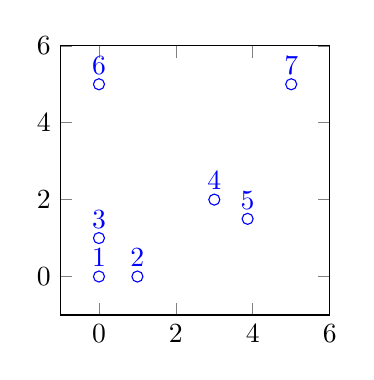
\begin{tikzpicture}
        \begin{axis}[
            ymin=-1,
            ymax=6,
            xmin=-1,
            xmax=6,
            width=5cm,
            height=5cm
        ]
            \addplot[
	            scatter,
                blue,
                nodes near coords,
                only marks,
                point meta=explicit symbolic,
                mark=o
            ]
                table[
                    x=x,
                    y=y,
                    meta=name,
                ] {
                    x     y   name
                    0    0    1
                    1    0    2
                    0    1    3
                    3    2    4
                    3.86602540378    1.5    5
                    0    5    6
                    5    5    7
                
                } coordinate [pos=0/6] (1)
                coordinate [pos=1/6] (2)
                coordinate [pos=2/6] (3)
                coordinate [pos=3/6] (4)
                coordinate [pos=4/6] (5)
                coordinate [pos=5/6] (6)
                coordinate [pos=6/6] (7);
        \end{axis} 
    \end{tikzpicture}
\end{document}
